% !TEX root = ../Ausarbeitung.tex
\section{Introduction}
\label{sec:intro}
In scope of the \textit{Praktikum} within the Human Brain Project, we work with the Neurorobotics Platform (NRP) which provides a simulation environment for robotics.
More specifically, our experiment setup consists of a table, on which a robot arm is placed.
The robot arm has six joints and a hand with five fingers.
In front of the robot arm, a cylinder is placed on the table.
The goal of the Praktikum is to move the cylinder as far as possible with the robot arm.
This can be performed by just hitting the cylinder away or by grabbing the cylinder and throwing it as far as possible.
The performance is measured by the distance of the cylinder from the table.
The setup is depicted in \autoref{fig:hbbprak_2018}.

In the following, several strategies to fulfill this task are presented.
To begin with, fundamentals of evolutionary algorithms and spiking neural network are explained in \autoref{sec:ea} respectively \autoref{sec:spiking}.
Subsequently, a hard-coded approach in \autoref{sec:hard-coded} followed by a more sophisticated learning approach with evolutionary algorithms in \autoref{sec:learned} is presented to solve the challenge.
Then, \autoref{sec:problems} depicts some obstacles that arose during the experiments and the Praktikum.
Finally, the results are presented in \autoref{sec:results} and a conclusion is drawn in \autoref{sec:conclusion}

\begin{figure}[h]
\centering
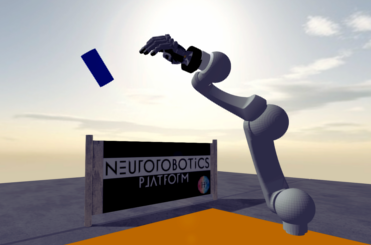
\includegraphics[width=.95\columnwidth]{figures/hbpprak_2018.png}
\caption{The goal is to throw the cylinder as far as possible.}
\label{fig:hbbprak_2018}
\end{figure}